%!TEX program = xelatex
%windows、macOS用户都可用
\documentclass[UTF8, punct, oneside, fontset=none]{ctexbook}
\usepackage[windows]{nsfc}
%macOS用户独享
%\documentclass[UTF8, punct, oneside]{ctexbook}
%\usepackage[macos]{nsfc}
%用来对比模版有无变化。对比时,请注释掉以下语句:
% \renewcommand{\input}[1]{\vspace{\baselineskip}}
%如果你个人文件和文件夹以⚠︎开头进行命名,可以省心更新模版。参见README.md

\pagestyle{empty} % 第二页以后页码空白
\usepackage[a4paper, left = 3.05cm, right = 3.05cm, top = 2.72cm, bottom = 2.54cm]{geometry}%页边距

\usepackage{times}

\usepackage{setspace}

\usepackage{comment}

\usepackage{pgfgantt}

\graphicspath{{figures/}}   % 设置图片所存放的目录
\begin{document}
%\thispagestyle{empty}    % 首页页码空白

{\centering\zhkai\fontsize{16pt}{21pt}\selectfont
\setlength{\baselineskip}{21pt}%最后设置,防止被fontsize中的覆盖
\hspace{30pt}\textbf{报告正文}\par
\vspace{5.46pt}}%0.2(行距倍数)*21(行距)*1.3(word)

%\begin{comment}
{\zhkai\fontsize{14pt}{22pt}\selectfont
 \setlength{\baselineskip}{22pt}%最后设置,防止被fontsize中的覆盖
参照以下提纲撰写,要求内容翔实、清晰,层次分明,标题突出。
\textbf{\color{YSFblue}请勿删除或改动下述提纲标题及括号中的文字。}\par
\vspace{1.3pt}}%0.5(行距倍数)*22(行距)*1.3(word)
%\end{comment}

\chapter{\textbf{立项依据与研究内容(建议8000字以下):}}
\vspace{4pt}
\section{\textbf{项目的立项依据}(研究意义、国内外研究现状及发展动态分析,需结合科学研究发展趋势来论述科学意义;\kg{0.2em}或结合国民经济和社会发展中迫切需要解决的关键科技问题来论述其应用前景。\kg{0.2em}附主要参考文献目录);}

\begin{MS}
	
\subsection{研究意义}
波动方程是二阶双曲型偏微分方程\cite{bedford1994},可用于描述地震波、水波、电磁波等自然界中的波动现象,广泛的应用于无损检测、地震预测、生物医学成像等各个工程领域。
发展波动方程的高精度分析方法将有助于提升如无损检测准确率、医学成像精度等。
由于实际工程问题中通常涉及复杂几何区域、材料非均质等一系列问题,采用理论分析手段研究波动问题难以获得解析解。于是,数值仿真分析成为了研究波动方程的重要工具。
在波动问题的主流数值分析方法中,时间域和空间域将独立离散为有限个分布节点用于近似位移变量,其中空间域通常采用基于变分原理的弱形式进行离散分析,如有限元法等。
在变分原理的帮助下,基于弱形式型的方法具有求解精度高、稳定性强的特点,适用于复杂空间几何构型。
而时间域则采用基于微分方程的强形式进行离散分析,如有限差分法等。
该类方法通常采用迭代形式进行程序实现,实现过程简单高效。
但基于强形式型的方法在计算精度和稳定性方面均低于基于弱形式型的方法,计算误差将随着迭代步的增加而累积增大。

波动方程数值分析方法构建的另一种思路是将时间域作为第四维空间,与时空间域进行混合离散,并采用基于哈密顿变分原理的弱形式进行求解。
该类方法将提升整体的求解精度,有利于时空区域自适应节点加密过程。
求解过程无需进行迭代,可采用整体并行计算求解提高效率。
然而自上世纪九十年代Hughes首次采用时空混合离散结合间断伽辽金法求解波动问题\cite{hughes1988}以来,该类方法发展缓慢。
\textbf{
主要的原因是该方法并不能适用于任意节点分布情况,导致其未能广泛应用于复杂的实际工程问题中,阻碍了时空混合离散伽辽金法的发展。
}
造成时空混合离散伽辽金法无法适用任意节点分布情况的原因主要有三点:

首先是\textbf{时域末端虚位移本质边界条件的施加问题}。
波动方程的时空混合离散伽辽金法通过哈密顿变分原理建立相对应的弱形式,
如图 \ref{fg:hamilton} 所示,哈密顿原理要求虚位移$\delta q$在初始时刻$t_0$和末端时刻$t_1$为零,即$\delta q(t_0)=\delta q(t_1)=0$,以等价于欧拉--拉格朗日方程\cite{arnold1978}。
在传统边值问题中,虚位移本质边界条件通常伴随着位移本质边界条件。
当采用伽辽金法进行求解时,即虚位移和位移采用相同的离散方式,位移及其虚位移涉及本质边界条件的自由度数量相同。
采用矩阵压缩技术直接施加本质边界条件时,可保持刚度矩阵为方阵且可逆。
然而,波动方程在时间维度上属于初值问题,即已知初始时刻位移和速度,$q(t_0)=q_0,\dot q(t_0) = \dot q_0$,时域末端边界条件未知。
如图 \ref{fg:direct} 所示,直接施加初始时刻位移边界条件将填补末端时刻虚位移为零造成刚度矩阵却是的部分。
而初始时刻虚位移不再要求为零,初始时刻速度边界条件可在此处作为自然边界条件施加。
但该方法可实施的前提是\textbf{涉及初始时刻和末端时刻的自由度数量需要保持一致,并不适用于任意节点分布情况。}
间断伽辽金法则是在弱形式中增加了哈密顿原理时域边界条件相关项,以规避虚位移本质边界条件的施加。
但是,该方法需要在时域上采用如图 \ref{fg:slab} 所示的分块离散以保证整体求解稳定性。
\textbf{时域分块网格不仅限制了节点布置,而且在时域块状边界处采用非连续的位移进行近似,增加位移自由度数量。}


\begin{figure}[!h]
    \centering 
    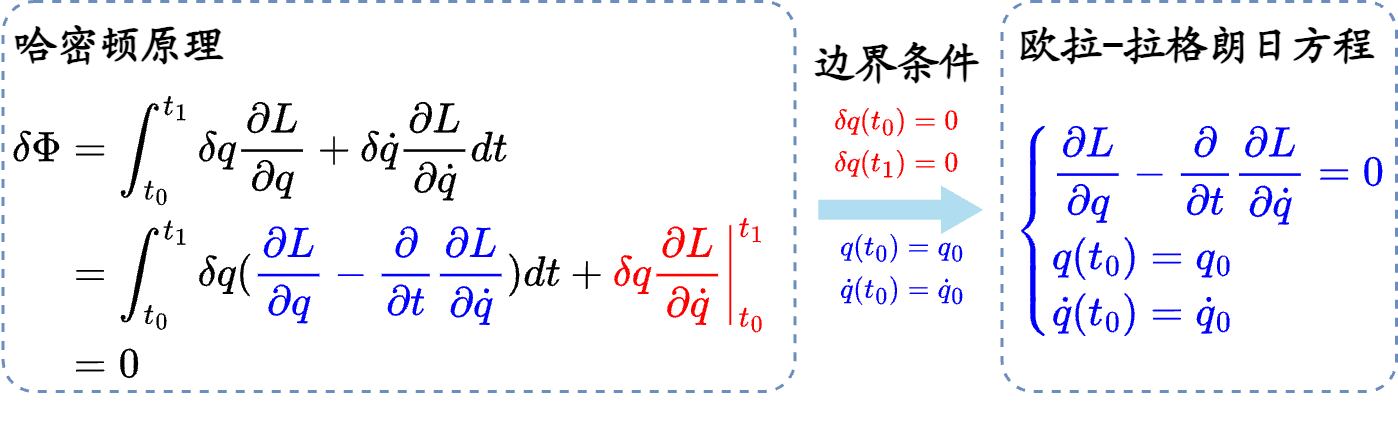
\includegraphics[width=\textwidth]{figures/Hamilton.png}
    \caption{哈密顿原理与欧拉--拉格朗日方程等价性}
    \label{fg:hamilton}
\end{figure}

\begin{figure}[!h]
    \centering 
    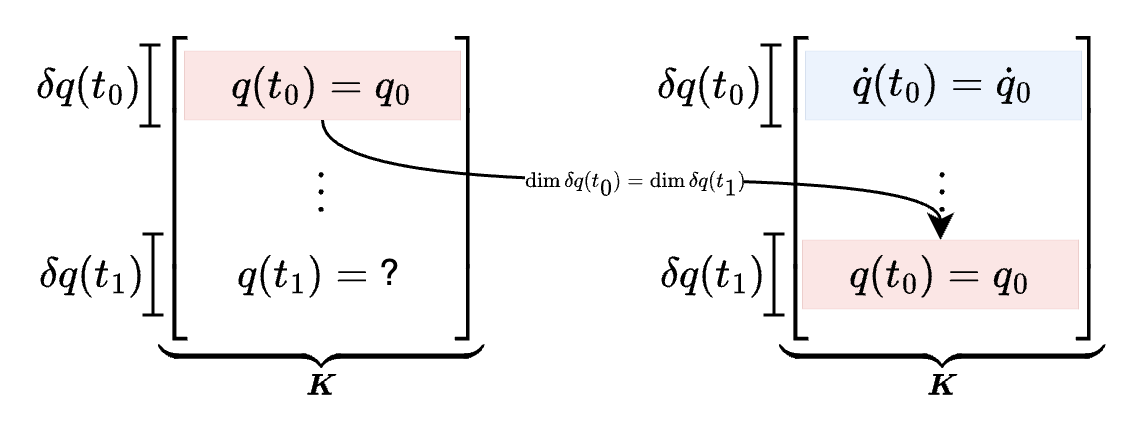
\includegraphics[width=0.8\textwidth]{figures/stiffness.png}
    \caption{直接施加时域末端虚位移本质边界条件}
    \label{fg:direct}
\end{figure}

\begin{figure}[!h]
    \centering 
    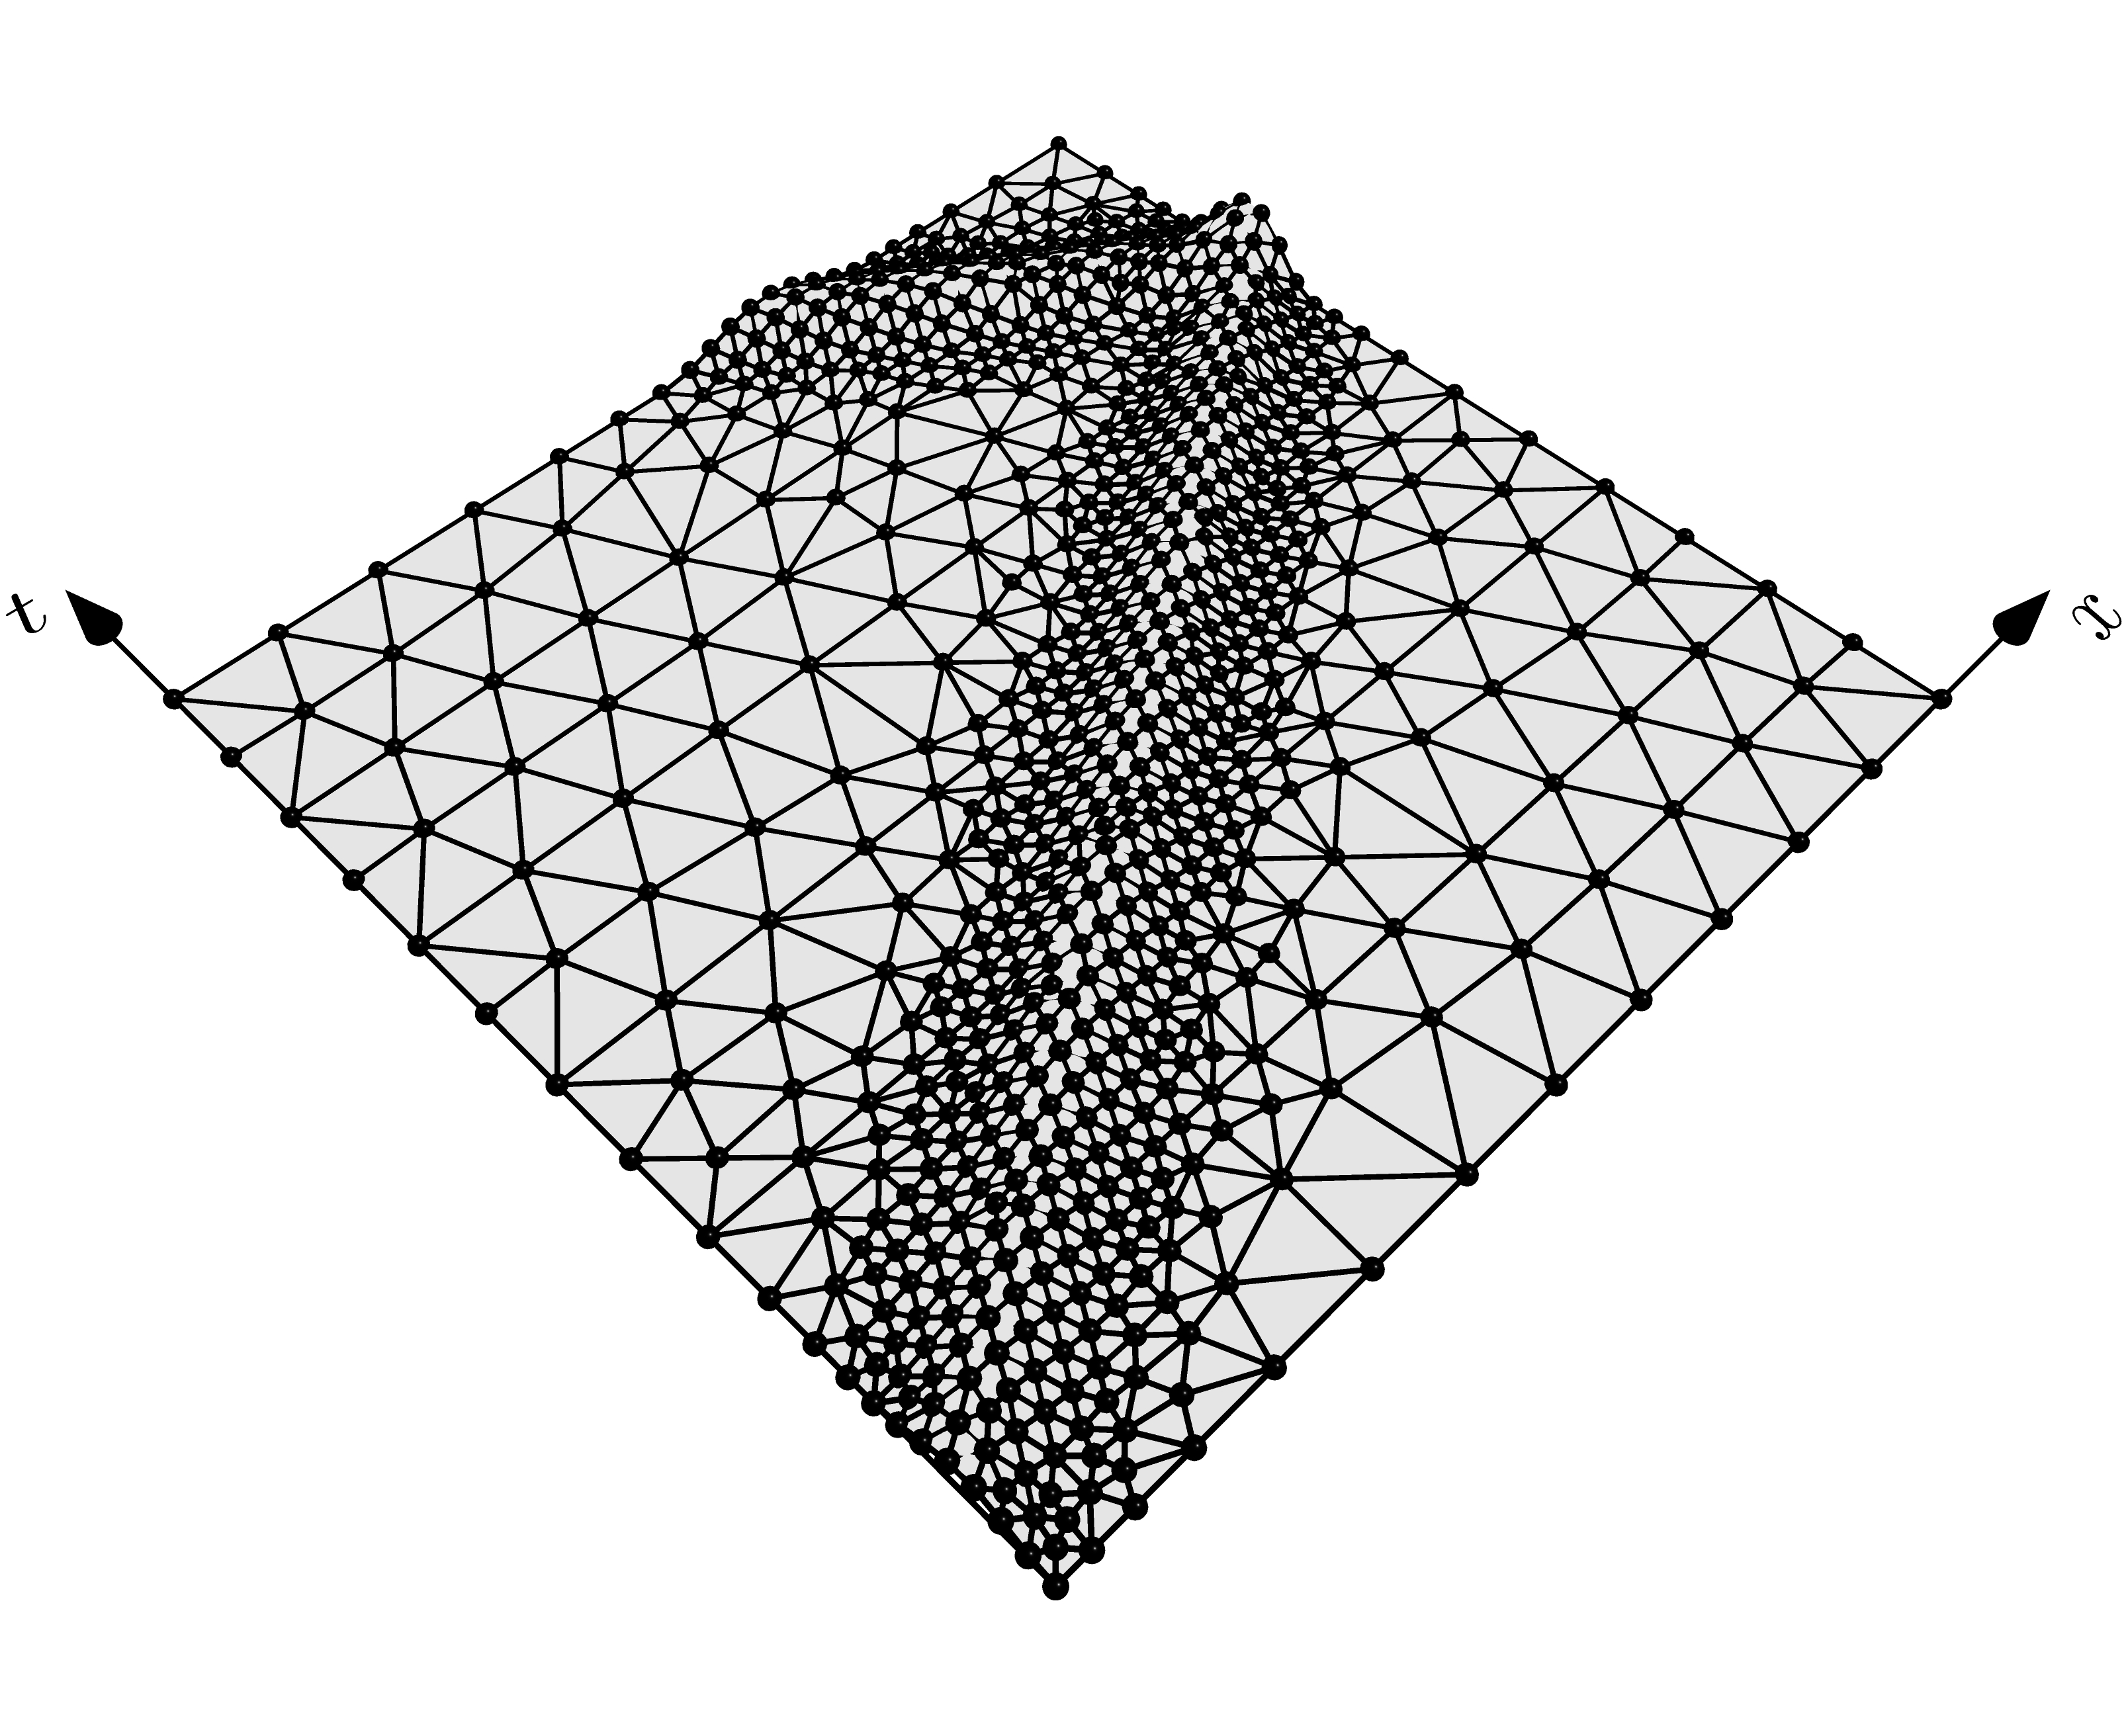
\includegraphics[width=0.8\textwidth]{figures/wave.png}
    \caption{时空混合离散间断伽辽金法}
    \label{fg:slab}
\end{figure}

% \begin{equation*}
% \begin{split}
% 	\delta \Phi&=\int_{t_0}^{t_1} \delta q \frac{\partial L}{\partial q} + \delta \dot q \frac{\partial L}{\partial \dot q} dt\\ &=\int_{t_0}^{t_1} \delta q({\color{blue}\frac{\partial L}{\partial q} - \frac{\partial}{\partial t}\frac{\partial L}{\partial \dot q}}) dt + {\color{red}\delta q \left . \frac{\partial L}{\partial \dot q}\right \vert_{t_0}^{t_1}}\\&= 0
% \end{split}
% \xrightarrow{{\color{red}\delta q(t_0)=\delta q(t_1)=0}}
% \color{blue}\left \{\begin{split}&\frac{\partial L}{\partial q} - \frac{\partial}{\partial t}\frac{\partial L}{\partial \dot q}=0\\& q(t_0) = q_0,\;\dot q(t_0) = \dot q_0\end{split}\right .
% \end{equation*}

其次是\textbf{空间域和时间域离散节点间距不匹配引起的数值色散问题}。

发展适用于任意节点分布的时空混合离散伽辽金法……

本项目

\subsection{国内外研究现状及发展动态}

\vspace{-5pt}

\begin{REF}
	\subsection*{参考文献}
	\vspace{-50pt}
	\bibliographystyle{gbt7714-2005-numerical}
	\bibliography{ref}%参考文献
\end{REF}

\newpage%自己判断是否需要

\end{MS}


\section{\textbf{项目的研究内容、研究目标,以及拟解决的关键科学问题}(此部分为重点阐述内容)\textbf{;}}

\begin{MS}
	\subsection{研究内容}
本项目将围绕波动方程中时空混合离散伽辽金法存在的问题,
研究时域末端虚位移本质边界条件施加方案,
构建可缓解数值色散问题的时空混合离散无网格近似方案,
并引入变分一致型伽辽金无网格数值积分法,
建立绝对时空混合离散伽辽金无网格分析方法。
具体的研究内容如下:

\subsubsection*{\bfseries (1)适用于任意节点离散的时域末端虚位移本质边界条件施加方案}
在波动方程哈密顿原理的基础上,分析能量泛函中时域末端虚位移本质边界条件下位移变量的求解空间。
将传统能量泛函中的虚位移作为拉格朗日乘子,设计全新拉格朗日乘子型能量泛函。
分析新建立的能量泛函中,经过拉格朗日乘子法投影后的位移变量空间与原空间的等价性。
同时在全新的能量泛函中引入应力边界条件与初始时刻动量边界条件,验证相对应拉格朗日乘子型伽辽金弱形式的变分一致性,证明其与欧拉--拉格朗日方程的等价性。


\subsubsection*{\bfseries (2)适用于波动方程的时空混合离散再生核无网格近似方案}
探究拉格朗日乘子型能量泛函的稳定性条件,构建考虑时空混合离散阶次的局部截断误差估计表达式。
研究考虑时间维度的再生核无网格近似框架,以时空混合离散截断误差估计为基础,确定误差稳定时的再生核近似基向量中时间维度相关单项式。
根据确定基向量表达式,调整再生核近似中核函数影响域大小和表达式,以确保再生核近似中矩量矩阵可逆。
最后,通过数值算例验证所提无网格近似方案能否缓解数值色散问题。

\subsubsection*{\bfseries (3)时空混合离散下变分一致型伽辽金无网格数值积分方案}
根据时空混合离散无网格近似中基向量的元素,确定波动问题拉格朗日乘子型伽辽金弱形式的积分约束条件。
以再生光滑梯度理论框架为基础,构建时空混合离散下满足积分约束条件的变分一致型伽辽金无网格数值积分方法。
在四维情况下,引入四面体柱或六面体柱单元作为背景积分域。通过再生光滑梯度的一致性条件,优化全局数值积分点数量,确定积分点位置和权重。
最后,通过时空混合离散分片试验,测试所提伽辽金无网格数值积分方案的变分一致性和计算精度。

\subsubsection*{\bfseries (4)绝对时空混合离散高效伽辽金无网格分析方法}
将时空混合离散再生核无网格近似引入拉格朗日乘子型伽辽金弱形式,结合变分一致型伽辽金无网格数值积分方案,建立波动方程时空混合离散控制方程。
进一步分析离散控制方程表达式,利用离散控制方程刚度矩阵的相识性,优化程序结构,降低内存开销。
同时,基于位移解的梯度变化,制定相对应的无网格自适应节点加密方案。
在求解离散控制方程时引入成熟并行计算库,实现时间域和空间域同时并行计算,
建立绝对时空混合离散高效伽辽金无网格分析方法及其通用数值仿真程序。通过典型波动问题和实际工程算例验证所提方法的有效性和可靠性。

\subsection{研究目标}
本项目完成上述各项研究内容旨在建立绝对时空混合离散伽辽金无网格分析方法,该方法能适用于任意布置的节点离散情况,缓解数值色散问题,
提升分析波动问题时的计算效率和稳定性。具体的研究目标包括:
\begin{enumerate}[label={\rmfamily (\theenumi)},left=24pt]
    \item 建立适用于任意节点离散的时域末端虚位移本质边界条件施加方案,提升时空混合离散伽辽金法对节点离散的鲁棒性;
    \item 提出适用于波动方程再生核无网格近似方案,缓解波动问题时空混合离散伽辽金无网格法的色散问题;
    \item 设计适用于高维波动方程的变分一致型伽辽金无网格法数值积分方案,提升时空混合离散伽辽金无网格法的计算效率;
    \item 发展绝对时空混合离散高效伽辽金无网格分析方法,为实际波动问题提供可靠、稳定的数值工具。
\end{enumerate}

\subsection{拟解决的关键科学问题}

本项目拟解决的关键科学问题如下:

\subsubsection*{\bfseries (1)如何在时空混合离散弱形式中施加时域末端虚位移本质边界条件}
哈密顿原理要求时域末端虚位移等于零,才可使相对应的弱形式等价于欧拉--拉格朗日方程。
由于在实际问题中,时域末端边界条件通常是未知的。单独令时域末端虚位移为零将导致整体弱形式丧失变分一致性,计算结果将出现与实际不符的情况。
目前已有方法通常是采用间断伽辽金格式规避时域末端边界,但需要采用分块网格技术提高求解的稳定性。
因此,如何正确施加时域末端虚位移本质边界条件,使时空混合离散伽辽金法适用于任意节点离散情况,是本项目研究内容(1)的关键科学问题。

\subsubsection*{\bfseries (2)如何确定时空混合无网格近似基向量阶次对求解稳定性的影响机理}
波动方程属于二阶双曲型偏微分方程,求解过程中时域离散节点间距过大将引起数值色散问题,导致计算结果发散。
传统方法可减小离散节点间距缓解该问题,随之将伴随自由度的增加所引起的计算量增大,不适合任意节点离散情况。
增加稳定项也可提升计算的稳定性,但节点间距过小时该方法将出现数值耗散问题,也不适用于任意节点离散情况。
本项目的研究内容(2)旨在利用无网格构造高阶再生特性形函数的便利性,缓解数值色散问题。因此,确定时空混合离散无网格近似基向量阶次对求解稳定性的影响机理,是该研究内容的关键科学问题。

\subsubsection*{\bfseries (3)如何优化时空混合离散变分一致伽辽金无网格数值积分方案}
由于无网格形函数通常为有理式,伽辽金无网格法需要采用变分一致型数值积分方案以保证计算精度。
变分一致型数值积分方案可通过形函数导数的一致性条件,优化全局数值积分点个数。
最终的数值积分点个数将直接影响时空混合离散伽辽金无网格法的计算效率。
相较于传统时间域与空间域分别离散的方法,时空混合离散将增加时间维度的离散,离散维度比传统方式增加了一个维度。
采用变分一致型伽辽金无网格数值积分方案时,需要额外考虑与时间维度相关的单项式积分约束条件与一致性条件。然而,为了缓解数值色散问题,时间维度相关的单项式阶次将不同于空间维度相关的单项式阶次。
如何在时空混合离散情况下优化变分一致型伽辽金无网格数值积分方案,提升整体计算效率,是本项目研究内容(3)的关键科学问题。


\end{MS}

\section{\textbf{拟采取的研究方案及可行性分析}\kg{0.3em}(\kg{0.1em}包括研究方法、\kg{0.2em}技术路线、实验手段、关键技术等说明);}

\begin{MS}
	%公式的上下间距
\setlength{\abovedisplayskip}{0pt}
\setlength{\belowdisplayskip}{0pt}

\subsection{研究方法与技术路线}

本项目将采用理论推导结合数值验证的方法进行研究,
首先,

具体的技术路线图如下所示。

\subsection{研究方案}

\subsubsection*{\bfseries (1)适用于任意节点离散的时域末端虚位移本质边界条件施加方案}
首先,查阅基于哈密顿变分原理时空混合离散有限元法的相关文献,确定虚位移本质边界条件的几种可能性。
将不同虚位移边界的方法进行数值实现,对比计算结果的稳定性和精度。
确定稳定性最优情况下的虚位移空间$\tilde V_h$,相对应的变分问题为:
\begin{equation}
    \text{find} \; u_h \in V_h, \quad a(u_h, \delta u_h) = f(\delta u_h), \quad \forall \delta u_h \in \tilde V_h
    \label{eq:1}
\end{equation}
其中,$V_h$为位移空间,$a:V\times V \rightarrow \mathbb R$为双线性算子,$f:V\rightarrow \mathbb R$为线性算子。

随后,将式\eqref{eq:1}中的虚位移$\delta u_h$作为拉格朗日乘子,设计全新拉格朗日乘子型能量泛函:
\begin{equation}
    \text{find} \; u_h \in V_h,\; p_h \in \tilde V_h, \quad
    \left \{
    \begin{split} 
        -a(u_h, \delta u_h) + a(p_h, \delta u_h) = 0,\quad &\forall \delta u_h \in V_h \\
        a(u_h, \delta p_h) = f(\delta p_h),\quad &\forall \delta p_h \in \tilde V_h
    \end{split}
    \right .
    \label{eq:2}
\end{equation}
从上式可以看出,原本式\eqref{eq:1}中的变分问题作为约束条件施加在拉格朗日乘子型伽辽金问题的弱形式中,需进一步在验证两者之间的等价性。
当等价性成立,仅需要采用常规方法对$p_h$施加本质边界条件,即可实现式\eqref{eq:1}中施加虚位移本质边界条件的效果。
同时,引入分部积分公式对式\eqref{eq:2}进行推导,通过修正$u_h$和$p_h$的边界条件,使所提的拉格朗日乘子型伽辽金弱形式满足变分一致性,并证明其与欧拉--拉格朗日方程等价。

最后,采用均布的有限元离散从数值上与传统方法进行对比,验证其计算精度。并用分均布节点离散验证所提方法求解的稳定性。

\subsubsection*{\bfseries (2)适用于波动方程的稳定再生核无网格近似方案}
首先,借鉴von Neumann稳定性分析方法,在拉格朗日型能量泛函所对应的离散控制方程中引入特征解的傅立叶展开式。
同时引入无网格形函数一致性条件,推导均布节点离散下离散控制方程中通用行的局部截断误差估计$\epsilon$,
$\epsilon$应包含时间域节点间距$\Delta t$和空间域节点间距$\Delta x$相关的余项:
\begin{equation}
    \epsilon = O(\Delta t^{n_t}) + O(\Delta x^{n_x})
\end{equation}
其中,$n_t$和$n_x$分别为时间域和空间域的离散阶次。根据截断误差估计,确定空间域离散阶次为$n_x$时,消除数值色散影响所需的时间域离散阶次$n_t$。

随后,在再生核无网格近似的理论框架下,构造相对应阶次的无网格近似基向量$\boldsymbol p^{[n_x,n_t]}$:
\begin{equation}
    \boldsymbol p^{[n_x,n_t]}(x,t) = \left \{1, x, t, x^2, xt, t^2, \dots, x^{n_x}, x^{n_x-1}t, \dots, t^{n_t} \right \}^T
\end{equation}
并根据无网格形函数中矩量矩阵的可逆性,确定核函数影响域在时间维度和空间维度包含节点的个数。

% \begin{figure}[H]
%     \centering
    
% \end{figure}

最后,通过数值验证所提混合离散再生核无网格近似的一致性条件。并代入所提拉格朗日型能量泛函,通过时间域、空间域不同比例节点间距和非均布节点离散测试其是否缓解数值色散问题。

\subsubsection*{\bfseries (3)时空混合离散下变分一致型伽辽金无网格数值积分方案}
首先,根据时空混合离散无网格近似中基向量的元素,推导拉格朗日型伽辽金弱形式的积分约束条件。
引入申请人所提出的再生光滑梯度理论框架,构建满足满足积分约束条件无网格形函数再生光滑梯度,以形函数的一阶时间光滑导数为例,其表达式为:
\begin{equation}
    \tilde \Psi_{I,t}(\boldsymbol x) = \boldsymbol p^{[n_x,n_t - 1]}(\boldsymbol x) \boldsymbol G^{ - 1} \boldsymbol g_{tI}
\end{equation}
其中,$\boldsymbol G$为矩量矩阵,$\boldsymbol g_{tI}$为积分约束条件。再生光滑梯度能自动满足积分约束条件,适用于相对应阶次的高斯积分方案。

随后,为进一步提升计算效率,将根据再生光滑梯度的一致性条件和数值积分点在单元间的共享特性,优化数值积分点的位置和权重,减少全局数值积分点数量。特别是针对四维空间,拟采用四面体柱或六面体柱单元作为背景积分域进行数值积分,构建适合时空混合离散再生光滑梯度积分法的数值积分方案。

% \begin{figure}[H]
%     \centering
    
% \end{figure}

最后,通过分片试验验证所提数值积分方案是否满足变分一致性,同时利用典型波动问题测试其计算精度。

\subsubsection*{\bfseries (4)任意节点分布时空混合离散伽辽金无网格分析方法}
首先,将时空混合离散再生核无网格形函数及其光滑梯度引入拉格朗日乘子型伽辽金弱形式\eqref{eq:1}中,并采用优化的伽辽金无网格数值积分方案进行积分,得到相应的离散控制方程。
由式\eqref{eq:1} 可知,所提时空混合离散伽辽金弱形式中双线性算子均为同一算子,区别在于变量$u_h$和$p_h$所处的空间不一致。
造成空间不一致的原因在于$u_h$和$p_h$的本质边界条件不一致。当$u_h$和$p_h$采用相同的近似方式进行离散时,单独将施加本质边界条件部分的刚度矩阵分出,可得到如下所示离散控制方程:
\begin{equation}
    \begin{bmatrix} 
        \boldsymbol K + \boldsymbol K_{u} & \boldsymbol K \\
        \boldsymbol K & \boldsymbol K_{p} 
    \end{bmatrix} 
    \begin{Bmatrix}
        \boldsymbol u \\ \boldsymbol p
    \end{Bmatrix} =
    \begin{Bmatrix} \boldsymbol f_u \\ \boldsymbol f + \boldsymbol f_p \end{Bmatrix}
    \label{eq:3} 
\end{equation}
其中,$\boldsymbol K_u$和$\boldsymbol f_u$、$\boldsymbol K_p$和$\boldsymbol f_p$分别为施加与$u_h$和$p_h$相关的本质边界条件刚度矩阵和力向量。式\eqref{eq:3}中,刚度矩阵$\boldsymbol K$重复在三个地方使用,将利用该特点优化程序结构,降低内存开销。

同时,$u_h$与$p_h$的本质边界条件需要采用满足伽辽金法变分一致性的施加方案进行施加。本项目将在申请人所提基于Hellinger--Reissner原理伽辽金无网格本质边界条件施加方案的基础上,研究适用于拉格朗日乘子型时空混合离散伽辽金弱形式的变分一致型施加方案,确保全域的变分一致性。

随后,为进一步提升稳定性,将引入基于位移解梯度变化的自适应节点加密方案,对波的传播动态进行精确捕捉。同时,在求解离散控制方程时,拟嵌入基于Krylov子空间法的并行计算库,对程序进行提速。最后,通过典型波动问题和实际工程算例验证所提方法的有效性和可靠性。

\subsection{可行性分析}

初步测试

前期研究支持


\end{MS}

\section{\textbf{本项目的特色与创新之处;}}

\begin{MS}
	
本项目的特色与创新之处包括以下三点:

\begin{enumerate}[label=(\theenumi),left=24pt]
    \item 时域末端虚位移本质边界条件施加方案
    实现了基于弱形式施加虚位移本质边界条件,无需分块网格划分,即可保证求解的稳定性。同时始末节点也无需匹配个数,降低节点离散的要求。
    \item 时空混合离散无网格近似方案利用再生核近似构造高阶形函数的便利性,在任意节点离散情况下即可缓解数值色散问题。基于节点离散的再生核近似局部节点加密过程实现简单,无需考虑几何拓扑关系。
    \item 在时域末端虚位移本质边界条件施加方案、时空混合离散无网格近似方案的协同作用下,时空混合伽辽金无网格分析方法可适用于任意节点离散情况,并且能轻松地进行局部区域的节点加密,更好捕捉波动问题的局部特征。
\end{enumerate}



\end{MS}

\section{\textbf{年度研究计划及预期研究结果}(包括拟组织的重要学术交流活动、国际合作与交流计划等)。}

\begin{MS}
	\subsection{年度研究计划}
本项目的年度研究计划如下:

% \textbf{2026年1月 -- 2026年12月:}
% 研究适用于任意节点离散的时域末端虚位移本质边界条件施加方案,
% 本年度计划参加国内学术会议2人次。

% \textbf{2027年1月 -- 2027年12月:}

% \textbf{2028年1月 -- 2028年12月:}

% \textbf{2029年1月 -- 2029年12月:}
\begin{table}[h!]
\caption{年度研究计划}
\centering
\begin{ganttchart}[
    x unit=8pt,
    vgrid,
    newline shortcut=true,
    bar label node/.append style={align=left}
]{1}{32}
    \gantttitle{2026}{8}
    \gantttitle{2027}{8}
    \gantttitle{2028}{8}
    \gantttitle{2029}{8} \\
    \gantttitle{上半年}{4}
    \gantttitle{下半年}{4}
    \gantttitle{上半年}{4}
    \gantttitle{下半年}{4}
    \gantttitle{上半年}{4}
    \gantttitle{下半年}{4}
    \gantttitle{上半年}{4}
    \gantttitle{下半年}{4} \\
    \ganttgroup{研究内容(1)}{1}{4} \\
    \ganttbar{时域末端虚位移本质边界条件施加方案}{1}{4} \\
    \ganttbar{时空混合离散误差估计}{1}{4} \\
    \ganttbar{时空混合离散误差估计}{1}{4} \\
    \ganttbar{成果整理、论文发表、\\软件著作权申请、年度\\报告及项目结题报告}{5}{32} \\
    % \ganttlinkedbar{Task 2}{3}{7} \ganttnewline
    % \ganttmilestone{Milestone}{7} \ganttnewline
    % \ganttbar{Final Task}{8}{12}
    % \ganttlink{elem2}{elem3}
    % \ganttlink{elem3}{elem4}
\end{ganttchart}
\end{table}

\subsection{预期研究结果}
本项目预期取得如下研究结果:

\begin{enumerate}[label=(\theenumi),left=24pt]
    \item 时空混合离散伽辽金法时域末端本质边界条件施加方案;
    \item 免数值色散问题的时空混合离散再生核无网格近似方案;
    \item 绝对混合离散高效伽辽金无网格分析方法;
    \item 在计算力学领域重要期刊发表论文5--9篇,申请软件著作权1项;
    \item 培养研究生不少于4名。
\end{enumerate}

\end{MS}

\chapter{\textbf{研究基础与工作条件}}
\section{\textbf{研究基础}(与本项目相关的研究工作积累和已取得的研究工作成绩);}

\begin{MS}
	

项目申请人主要从事伽辽金无网格法相关领域研究,并取得了一定的研究成果,已有国内外计算力学领域重要期刊发表论文20余篇,其中5篇发表于\textit{Computer Methods in Applied Mechanics and Engineering}。
相关系列工作不仅为本项目的研究奠定了坚实的研究基础,并积累了丰富的理论分析经验。具体表现为:

(1)fs

\begin{lstlisting}[language=tex, basicstyle=\ttfamily\tiny, keywordstyle=\color{blue}, commentstyle=\color{gray}]
	\begin{thebibliography}{1}
		\bibitem{test}
		\bibauthor{\textbf{C\"aldognetto T\@, Tenti P}}\@. 
		\bibtitle{Microgrids Operation Based on Master–Slave Cooperative Control}
		\bibmark{[J]}\@.
		\bibjournal{IEEE Journal of Emerging and Selected Topics in Power Electronics}\@,
		\bibvolume{2}\bibnumber{(4)}\thinspace{}\textnormal{:}
		\bibpages{1081\thinspace{}\textnormal{--}\thinspace{}1088}\@,
		\bibyear{2014}\@.
		\url{doi: 10.1109/JESTPE.2014.2345052}\@.
	\end{thebibliography}
\end{lstlisting}

\vspace{-50pt}
\begin{thebibliography}{1}
	\providecommand{\bibauthor}[1]{#1}
	\providecommand{\bibeditor}[1]{#1}
	\providecommand{\bibtranslator}[1]{#1}
	\providecommand{\bibtitle}[1]{#1}
	\providecommand{\bibbooktitle}[1]{#1}
	\providecommand{\bibjournal}[1]{#1}
	\providecommand{\bibmark}[1]{#1}
	\providecommand{\bibcountry}[1]{#1}
	\providecommand{\bibpatentid}[1]{#1}
	\providecommand{\bibedition}[1]{#1}
	\providecommand{\biborganization}[1]{#1}
	\providecommand{\bibaddress}[1]{#1}
	\providecommand{\bibpublisher}[1]{#1}
	\providecommand{\bibinstitution}[1]{#1}
	\providecommand{\bibschool}[1]{#1}
	\providecommand{\bibvolume}[1]{#1}
	\providecommand{\bibnumber}[1]{#1}
	\providecommand{\bibversion}[1]{#1}
	\providecommand{\bibpages}[1]{#1}
	\providecommand{\bibmodifydate}[1]{#1}
	\providecommand{\bibcitedate}[1]{#1}
	\providecommand{\bibyear}[1]{#1}
	\providecommand{\bibdate}[1]{#1}
	\providecommand{\biburl}[1]{\newline\url{#1}}
	\bibitem{test}
	\bibauthor{\textbf{C\"aldognetto T\@, Tenti P}}\@. \bibtitle{Microgrids Operation Based
		on Master–Slave Cooperative Control}\bibmark{[J/OL]}\@. \bibjournal{IEEE
		Journal of Emerging and Selected Topics in Power Electronics}\@,
	\bibvolume{2}\bibnumber{(4)}\thinspace{}\textnormal{:
	}\bibpages{1081\thinspace{}\textnormal{--}\thinspace{}1088}\@,
	\bibyear{2014}\@. \url{doi: 10.1109/JESTPE.2014.2345052}\@.
\end{thebibliography}
\end{MS}

\section{\textbf{工作条件}(包括已具备的实验条件,尚缺少的实验条件和拟解决的途径\kg{0.2em},包括利用国家实验室、\kg{0.2em}全国重点实验室和部门重点实验室等研究基地的计划与落实情况);}

\begin{MS}
	本项目依托华侨大学土木工程学院及福建省智慧基础设施与监测重点实验室(华侨大学)进行,实验室包括

华侨大学
\end{MS}

\section{\textbf{正在承担的与本项目相关的科研项目情况}(申请人和主要参与者正在承担的与本项目相关的科研项目情况,\kg{0.18em}包括国家自然科学基金的项目和国家其他科技计划项目,要注明项目的资助机构、项目类别、批准号、\kg{0.1em}项目名称、\kg{0.1em}获资助金额、\kg{0.1em}起止年月、\kg{0.1em}与本项目的关系及负责的内容等);}

\begin{MS}
	\input{sections/二3正承担}
\end{MS}


\section{\textbf{完成国家自然科学基金项目情况}(对申请人负责的前一个已资助期满的科学基金项目\kg{0.15em}(项目名称及批准号)\kg{0.15em}完成情况、\kg{0.15em}后续研究进展及与本申请项目的关系加以详细说明。\kg{0.3em}另附该项目的研究工作总结摘要(限500字)和相关成果详细目录)。}

\begin{MS}
	\input{sections/二4已完成}
\end{MS}

\chapter{\textbf{其他需要说明的情况}}
\section{申请人同年申请不同类型的国家自然科学基金项目情况(列明同年申请的其他项目的项目类型、\kg{0.2em}项目名称信息,\kg{0.2em}并说明与本项目之间的区别与联系;已收到自然科学基金委不予受理或不予资助决定的, 无需列出)。}

\begin{MS}
	\input{sections/三1同年申请}
\end{MS}

\section{具有高级专业技术职务\kg{0.2em}(职称)\kg{0.2em}的申请人或者主要参与者是否存在同年申请或者参与申请国家自然科学基金项目的单位不一致的情况;\kg{0.1em}如存在上述情况,\kg{0.1em}列明所涉及人员的姓名,\kg{0.1em}申请或参与申请的其他项目的项目类型、\kg{0.2em}项目名称、\kg{0.2em}单位名称、\kg{0.2em}上述人员在该项目中是申请人还是参与者,并说明单位不一致原因。}

\begin{MS}
	\input{sections/三2同年不一致}
\end{MS}

\section{具有高级专业技术职务\kg{0.2em}(职称)\kg{0.2em}的申请人或者主要参与者是否存在与正在承担的国家自然科学基金项目的单位不一致的情况;\kg{0.2em}如存在上述情况,列明所涉及人员的姓名,\kg{0.2em}正在承担项目的批准号、\kg{0.2em}项目类型、\kg{0.2em}项目名称、单位名称、起止年月,并说明单位不一致原因。}

\begin{MS}
	\input{sections/三3已有不一致}
\end{MS}

\section{同年以不同专业技术职务\kg{0.2em}(职称)\kg{0.2em}申请或参与申请科学基金项 目的情况(应详细说明原因)。}

\begin{MS}
	\input{sections/三4同年不同职务}
\end{MS}

\section{其他。}

\begin{MS}
	\input{sections/三5其他}
\end{MS}

\end{document}
